% !TEX program = xelatex

% 模板名称: 双栏硕博论文模板 
% 
% 注意: 这个模板使用了<fontspec>宏, 这个宏只能使用xelatex编译器来编译.
%
% 测试日期: 2025.1.8
\documentclass[a4paper, UTF8]{ctexart}

% \usepackage[comma,numbers,square,sort&compress]{natbib}
\usepackage{amsmath}
\usepackage[linesnumbered, ruled, lined,boxed,commentsnumbered]{algorithm2e}[1]
\usepackage{amssymb}
\usepackage{algorithmic}
\usepackage{fontspec} % 注意这个宏需要使用xelatex编译, 如果不需要这个宏, 可以直接注释掉
\usepackage{hhline}
% \usepackage{CTEX}
\usepackage{caption}
\usepackage{graphicx}   % 导入图片
\usepackage{epstopdf}
\usepackage{multicol}
\usepackage{multirow}
\usepackage{longtable}
\usepackage[subfigure,AllowH]{graphfig}
\usepackage[left=1.70cm, right=1.70cm, top=2.00cm, bottom=2.00cm]{geometry} %页边距

\usepackage[backend=biber]{biblatex}
\usepackage[colorlinks,linkcolor=blue,citecolor=blue,urlcolor=OliveGreen]{hyperref}
\usepackage[dvipsnames]{xcolor}

\addbibresource{books.bib}%须带参考文献库文件扩展名

\newenvironment{figurehere} 
{\def\@captype{figure}} 
\makeatother%用于连接公式编号

\begin{document}
	
	%------------------- 中文标题、作者、摘要和关键字
	\setlength{\columnwidth}{17.6cm}
	
	\title{基于XXXX优化研究}
	
	\author{小明\\ XX大学XX学院,学号}
	\date{2023.11.20}
	
	\maketitle
	\begin{center}  
		\parbox{\textwidth}{  {\heiti 摘~~~要:} {\kaishu 君不见,黄河之水天上来,奔流到海不复回。君不见,高堂明镜悲白发,朝如青丝暮成雪。人生得意须尽欢,莫使金樽空对月。天生我材必有用,千金散尽还复来。烹羊宰牛且为乐,会须一饮三百杯。岑夫子,丹丘生,将进酒,杯莫停。与君歌一曲,请君为我倾耳听。钟鼓馔玉不足贵,但愿长醉不复醒。古来圣贤皆寂寞,惟有饮者留其名。陈王昔时宴平乐,斗酒十千恣欢谑。主人何为言少钱,径须沽取对君酌。五花马、千金裘,呼儿将出换美酒,与尔同销万古愁。}\\  {\heiti 关键词:} {\kaishu 将进酒,将进酒,将进酒,李白}\\}  
	\end{center}
	\maketitle

	\cite{1}
			
	\footnotetext{将进酒 李白} %脚注
	
	\setlength{\columnsep}{0.7cm}\setlength{\columnwidth}{8.45cm}\begin{multicols}{2}
	
	\section{引言}% 第一章
	
	\subsection{研究背景}%1.1节
	
	君不见,黄河之水天上来,奔流到海不复回。君不见,高堂明镜悲白发,朝如青丝暮成雪。人生得意须尽欢,莫使金樽空对月。天生我材必有用,千金散尽还复来。烹羊宰牛且为乐,会须一饮三百杯。岑夫子,丹丘生,将进酒,杯莫停。与君歌一曲,请君为我倾耳听。钟鼓馔玉不足贵,但愿长醉不复醒。古来圣贤皆寂寞,惟有饮者留其名。陈王昔时宴平乐,斗酒十千恣欢谑。主人何为言少钱,径须沽取对君酌。五花马、千金裘,呼儿将出换美酒,与尔同销万古愁。
	
	\subsection{研究意义}%1.2节
	
	君不见,黄河之水天上来,奔流到海不复回。君不见,高堂明镜悲白发,朝如青丝暮成雪。人生得意须尽欢,莫使金樽空对月。天生我材必有用,千金散尽还复来。烹羊宰牛且为乐,会须一饮三百杯。岑夫子,丹丘生,将进酒,杯莫停。与君歌一曲,请君为我倾耳听。钟鼓馔玉不足贵,但愿长醉不复醒。古来圣贤皆寂寞,惟有饮者留其名。陈王昔时宴平乐,斗酒十千恣欢谑。主人何为言少钱,径须沽取对君酌。五花马、千金裘,呼儿将出换美酒,与尔同销万古愁。
	
	\begin{itemize}
		\item 满足实时性要求
		\item 满足实时性要求
		\item 满足实时性要求
	\end{itemize}
	
	\subsection{研究目的}%1.3节
	
	君不见,黄河之水天上来,奔流到海不复回。君不见,高堂明镜悲白发,朝如青丝暮成雪。人生得意须尽欢,莫使金樽空对月。天生我材必有用,千金散尽还复来。烹羊宰牛且为乐,会须一饮三百杯。岑夫子,丹丘生,将进酒,杯莫停。与君歌一曲,请君为我倾耳听。钟鼓馔玉不足贵,但愿长醉不复醒。古来圣贤皆寂寞,惟有饮者留其名。陈王昔时宴平乐,斗酒十千恣欢谑。主人何为言少钱,径须沽取对君酌。五花马、千金裘,呼儿将出换美酒,与尔同销万古愁。
	
	
	\section{关键技术}% 第二章
	
	\subsection{系统模型}%2.1节
	
	君不见,黄河之水天上来,奔流到海不复回。君不见,高堂明镜悲白发,朝如青丝暮成雪。人生得意须尽欢,莫使金樽空对月。天生我材必有用,千金散尽还复来。烹羊宰牛且为乐,会须一饮三百杯。岑夫子,丹丘生,将进酒,杯莫停。与君歌一曲,请君为我倾耳听。钟鼓馔玉不足贵,但愿长醉不复醒。古来圣贤皆寂寞,惟有饮者留其名。陈王昔时宴平乐,斗酒十千恣欢谑。主人何为言少钱,径须沽取对君酌。五花马、千金裘,呼儿将出换美酒,与尔同销万古愁。
	
	\begin{figurehere}  %替换掉之前的begin{figure}
		%由于分栏后图片不能显示出来,所以引用一个新的环境来添加图片
		%该环境已经在文章最开头定义好了
		\centering% 图片居中
		%\caption{系统模型符号}
		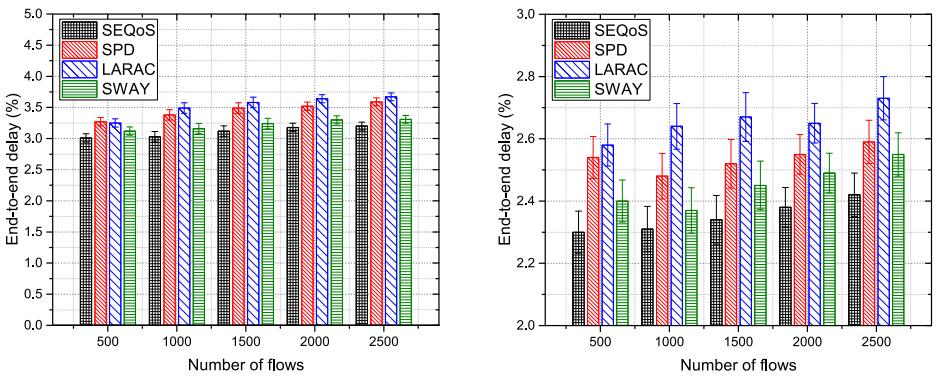
\includegraphics[width=8.5cm]{3.jpg}
		\label{1}
		\\\centerline{图1 系统模型符号}
	\end{figurehere}%替换掉之前的end{figure}

	君不见,黄河之水天上来,奔流到海不复回。君不见,高堂明镜悲白发,朝如青丝暮成雪。人生得意须尽欢,莫使金樽空对月。天生我材必有用,千金散尽还复来。烹羊宰牛且为乐,会须一饮三百杯。岑夫子,丹丘生,将进酒,杯莫停。与君歌一曲,请君为我倾耳听。钟鼓馔玉不足贵,但愿长醉不复醒。古来圣贤皆寂寞,惟有饮者留其名。陈王昔时宴平乐,斗酒十千恣欢谑。主人何为言少钱,径须沽取对君酌。五花马、千金裘,呼儿将出换美酒,与尔同销万古愁。

	\subsection{问题描述}%2.2节
	
	君不见,黄河之水天上来,奔流到海不复回。君不见,高堂明镜悲白发,朝如青丝暮成雪。人生得意须尽欢,莫使金樽空对月。天生我材必有用,千金散尽还复来。烹羊宰牛且为乐,会须一饮三百杯。岑夫子,丹丘生,将进酒,杯莫停。与君歌一曲,请君为我倾耳听。钟鼓馔玉不足贵,但愿长醉不复醒。古来圣贤皆寂寞,惟有饮者留其名。陈王昔时宴平乐,斗酒十千恣欢谑。主人何为言少钱,径须沽取对君酌。五花马、千金裘,呼儿将出换美酒,与尔同销万古愁。
	
	根据带宽消耗规则,一条路径的容量在数学上定义为:
	$$C(f_m)=\min_{(i,j)\in E}c(i,j)\alpha_m(i,j).$$
	
	其中,$(i,j)\in E$为所有数据流$f_m(j)\in F_L$流出的流量,令$C_r(i,j)$表示通过边缘路由的剩余带宽,定义为:
	$$C_r(i,j)=c(i,j)-\sum_{f_m\in E}q_k^\text{bandwidth}{ \alpha _ m }(i,j).$$
	
	\subsubsection{最大化流量问题}
	
	君不见,黄河之水天上来,奔流到海不复回。君不见,高堂明镜悲白发,朝如青丝暮成雪。人生得意须尽欢,莫使金樽空对月。
	
	$$\text{P2:}\max\sum_{f_m\in F_L}\sum_{(i,j)\in E}f_m\alpha(i,j). $$
	
	s.t. $C1-C4$
	
	\subsubsection{最小化成本问题}
	
	君不见,黄河之水天上来,奔流到海不复回。君不见,高堂明镜悲白发,朝如青丝暮成雪。人生得意须尽欢,莫使金樽空对月。天生我材必有用,千金散尽还复来。烹羊宰牛且为乐,会须一饮三百杯。岑夫子,丹丘生,将进酒,杯莫停。与君歌一曲,请君为我倾耳听。钟鼓馔玉不足贵,但愿长醉不复醒。古来圣贤皆寂寞,惟有饮者留其名。陈王昔时宴平乐,斗酒十千恣欢谑。主人何为言少钱,径须沽取对君酌。五花马、千金裘,呼儿将出换美酒,与尔同销万古愁。
	
	$$\text{P3:}\min\sum_{f_m\in F_L}\sum_{(i,j)\in E}f_mC(i,j)\beta(i,j). $$
	
	s.t. $C1-C4$
	
	\subsection{解决方法}%2.3节
	
	君不见,黄河之水天上来,奔流到海不复回。君不见,高堂明镜悲白发,朝如青丝暮成雪。人生得意须尽欢,莫使金樽空对月。天生我材必有用,千金散尽还复来。烹羊宰牛且为乐,会须一饮三百杯。岑夫子,丹丘生,将进酒,杯莫停。与君歌一曲,请君为我倾耳听。钟鼓馔玉不足贵,但愿长醉不复醒。古来圣贤皆寂寞,惟有饮者留其名。陈王昔时宴平乐,斗酒十千恣欢谑。主人何为言少钱,径须沽取对君酌。五花马、千金裘,呼儿将出换美酒,与尔同销万古愁。
		
	\renewcommand{\algorithmcfname}{算法}  %<---细节与重点
	\SetKwInput{KwIn}{输入}  %<---细节与重点
	\SetKwInput{KwOut}{输出}  %<---细节与重点
	\begin{algorithm}[H]
		\renewcommand{\thealgocf}{1}     %<---细节与重点
		\SetAlgoLined
		\KwIn{流$f_m$,每个流需要满足边的QoS要求 }
		\KwOut{流$f_m$的最短路径}
		流$f_m$转发至集合$S$\\
		$Pointer\gets 1$\\
		\While{$Pointer > 0$}
		{
			$Pointer > 0$\\
			更新路径$(S,E,Distance)$
		}	
		%\ForEach{$Pointer > 0$}
		%{
			%	\ForEach{$u_k \in \mathcal{W}_{v_i}  \left[ j-w : j +w  \right] $}
			%	{
				%		$J(\Phi) = - log P\left( u_k | \Phi  ( v_j) \right)$ \;
				%		$\Phi = \Phi - \alpha * \frac{\partial J}{\partial \Phi }$ \;		
				%	}
			%}  
		更新路径$(S,E,Distance,Previous)$\\
		计算流量最短路径,转发信息给$P$\\
		\caption{使用PyCUDA并行计算k条最短路径}
	\end{algorithm}		
	
	\begin{algorithm}[H]
		\renewcommand{\thealgocf}{2}     %<---细节与重点
		\SetAlgoLined
		\KwIn{有向图,$N$}
		\KwIn{一组流$f_m\in F_L$,每个流需要满足智能医疗应用的QoS要求}
		\KwIn{$ls$、$ds$、$js$流的优先级及相应的QoS要求}
		\KwIn{交换机最大规则容量$R_m(i)$}
		\KwOut{能够转发流不同QoS要求的边或路由的集合}
		\For{$j\in N$ and $S$}
		{
			初始化$flow-rules(j)\gets R_m$
		}	
		$k,k\gets 1$\\
		\While{所有流$f_m\in F_L$没有被转发}
		{
			$ls$、$ds$、$js$流公平分配\\
			\If{$ds$没有被转发}
			{
				\For{$m\gets 1$ to $C_1$}
				{
					搜索最优路由$(x_m,z_m,q_m,t_m)$
					$k\gets k+1$,满足$ds$流的QoS要求
				}
			}
			\If{$js$没有被转发}
			{
				\For{$n\gets 1$ to $C_2$}
				{
					搜索最优路由$(x_m,z_m,q_m,t_m)$
					$j\gets j+1$,满足$js$流的QoS要求
				}
			}
			\If{$ls$没有被转发}
			{
				\For{$q\gets 1$ to $C_3$}
				{
					搜索最优路由$(x_m,z_m,q_m,t_m)$
					$p\gets p+1$,满足$ls$流的QoS要求
				}
			}
		}	
		\caption{QoS路由算法,寻找最优路由}
	\end{algorithm}	
	
	君不见,黄河之水天上来,奔流到海不复回。君不见,高堂明镜悲白发,朝如青丝暮成雪。人生得意须尽欢,莫使金樽空对月。天生我材必有用,千金散尽还复来。烹羊宰牛且为乐,会须一饮三百杯。岑夫子,丹丘生,将进酒,杯莫停。与君歌一曲,请君为我倾耳听。钟鼓馔玉不足贵,但愿长醉不复醒。古来圣贤皆寂寞,惟有饮者留其名。陈王昔时宴平乐,斗酒十千恣欢谑。主人何为言少钱,径须沽取对君酌。五花马、千金裘,呼儿将出换美酒,与尔同销万古愁。
	
	
	\section{仿真分析}% 第三章	
	
	\subsection{在线方式性能比较}%3.2节
	
	\subsubsection{端到端时延}%3.2.1节
	
	君不见,黄河之水天上来,奔流到海不复回。君不见,高堂明镜悲白发,朝如青丝暮成雪。人生得意须尽欢,莫使金樽空对月。天生我材必有用,千金散尽还复来。烹羊宰牛且为乐,会须一饮三百杯。岑夫子,丹丘生,将进酒,杯莫停。与君歌一曲,请君为我倾耳听。钟鼓馔玉不足贵,但愿长醉不复醒。古来圣贤皆寂寞,惟有饮者留其名。陈王昔时宴平乐,斗酒十千恣欢谑。主人何为言少钱,径须沽取对君酌。五花马、千金裘,呼儿将出换美酒,与尔同销万古愁。
	
	\begin{figurehere}  
		\centering
		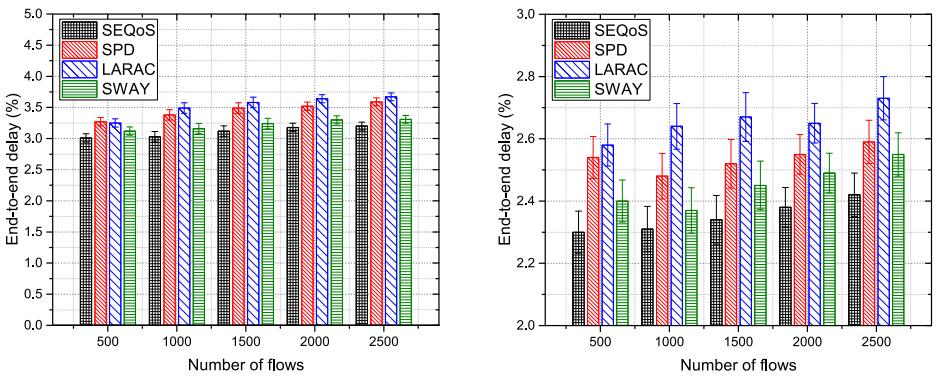
\includegraphics[width=8.5cm]{3.jpg}
		\label{3}
		\\\centerline{(a)使用AttMpls拓扑\quad(b)使用Goodnet拓扑}
		\centerline{图2 端到端时延\cite{ref1}}
	\end{figurehere}
	
	君不见,黄河之水天上来,奔流到海不复回。君不见,高堂明镜悲白发,朝如青丝暮成雪。人生得意须尽欢,莫使金樽空对月。天生我材必有用,千金散尽还复来。烹羊宰牛且为乐,会须一饮三百杯。岑夫子,丹丘生,将进酒,杯莫停。与君歌一曲,请君为我倾耳听。钟鼓馔玉不足贵,但愿长醉不复醒。古来圣贤皆寂寞,惟有饮者留其名。陈王昔时宴平乐,斗酒十千恣欢谑。主人何为言少钱,径须沽取对君酌。五花马、千金裘,呼儿将出换美酒,与尔同销万古愁。
	
	
	\section{总结}% 第四章
	
	\subsection{研究结论}%4.1节
	
	君不见,黄河之水天上来,奔流到海不复回。君不见,高堂明镜悲白发,朝如青丝暮成雪。人生得意须尽欢,莫使金樽空对月。天生我材必有用,千金散尽还复来。烹羊宰牛且为乐,会须一饮三百杯。岑夫子,丹丘生,将进酒,杯莫停。与君歌一曲,请君为我倾耳听。钟鼓馔玉不足贵,但愿长醉不复醒。古来圣贤皆寂寞,惟有饮者留其名。陈王昔时宴平乐,斗酒十千恣欢谑。主人何为言少钱,径须沽取对君酌。五花马、千金裘,呼儿将出换美酒,与尔同销万古愁。
	
	\subsection{优化讨论}%4.2节
	
	君不见,黄河之水天上来,奔流到海不复回。君不见,高堂明镜悲白发,朝如青丝暮成雪。人生得意须尽欢,莫使金樽空对月。天生我材必有用,千金散尽还复来。烹羊宰牛且为乐,会须一饮三百杯。岑夫子,丹丘生,将进酒,杯莫停。与君歌一曲,请君为我倾耳听。钟鼓馔玉不足贵,但愿长醉不复醒。古来圣贤皆寂寞,惟有饮者留其名。陈王昔时宴平乐,斗酒十千恣欢谑。主人何为言少钱,径须沽取对君酌。五花马、千金裘,呼儿将出换美酒,与尔同销万古愁。
	
	\end{multicols}

	\section*{主讲教师评分及评语:}


	\clearpage
	\printbibliography[heading=bibintoc,title=参考文献]%在目录列表中显示参考文献,title为自定义。
\end{document}
